\documentclass[pdftex,english,oribibl]{llncs}

%% Spracheinstellungen laden
\usepackage[english]{babel}

%% Schriftart in der Ausgabe/Eingabe
\usepackage[T1]{fontenc}
\usepackage{textcomp}
\usepackage[latin1]{inputenc}
\usepackage{comment}
%% Zitate
\usepackage[numbers]{natbib}
\bibliographystyle{abbrvnat}
%\bibliographystyle{dinat}
%\bibliographystyle{plainnat}
%\bibliographystyle{splncs}
%% Similar to option "sectionbib" but \refname instead of \bibname
\makeatletter
\renewcommand\bibsection{\section*{\refname\@mkboth{\MakeUppercase{\refname}}{\MakeUppercase{\refname}}}}
\makeatother

%% Index
%\usepackage{makeidx}
%\makeindex

%% PDF Einstellungen
% muss nach natbib geladen werden!
\usepackage{nameref}
\usepackage{varioref}
\usepackage[pdfusetitle,pdftex,colorlinks]{hyperref}
\hypersetup{pdfborder={0 0 0}}
\hypersetup{bookmarksdepth=3}
\hypersetup{bookmarksopen=true}
\hypersetup{bookmarksopenlevel=1}
\hypersetup{bookmarksnumbered=true}
\usepackage{color}
\hypersetup{colorlinks=false}

%\usepackage[section]{tocbibind}

\makeatletter
\gdef\@keywords{}
\def\keywords#1{\gdef\@keywords{#1}}
\gdef\@subtitle{}
\def\subtitle#1{\gdef\@subtitle{#1}}

%% modified from llncs
\renewenvironment{abstract}{%
  \list{}{\advance\topsep by0.35cm\relax\small%
          \leftmargin=1cm%
          \labelwidth=\z@%
          \listparindent=\z@%
          \itemindent\listparindent%
          \rightmargin\leftmargin}%
          \item[\hskip\labelsep\bfseries\abstractname]}{%
  \if!\@keywords!\else{\item[~]\item[\hskip\labelsep\bfseries\keywordname]\@keywords}\fi%
  \endlist}

\AtBeginDocument{%
  \if!\@subtitle!\else\hypersetup{pdfsubject={\@subtitle}}\fi
  \if!\@keywords!\else\hypersetup{pdfkeywords={\@keywords}}\fi
}
\makeatother

% llncs hyperref fix
\makeatletter
\providecommand*{\toclevel@author}{0}
\providecommand*{\toclevel@title}{0}
\makeatother

%% Grafiken
\usepackage[pdftex]{graphicx}
\DeclareGraphicsExtensions{.pdf,.jpg,.png}
\usepackage{subfigure}

%% Mathe
\usepackage{amsmath}
\usepackage{amssymb}

%% Listings
\usepackage{listings}
\lstset{escapechar=\%, frame=tb, basicstyle=\footnotesize}

%% Sonstiges
\newcommand{\TODO}[1]{\par\textcolor{red}{#1}\marginpar{\textcolor{red}{TODO}}}
\newcommand{\TODOX}[1]{\textcolor{red}{#1}\marginpar{\textcolor{red}{TODO}}}
\pagestyle{plain}

% Keine "Schusterjungen"
\clubpenalty = 10000
% Keine "Hurenkinder"
\widowpenalty = 10000 \displaywidowpenalty = 10000

%%%%%%%%%%%%%%%%%%%%%%%%%%%%%%%%%%%%%%%%%%%%%%%%%%%%%%%%%%%%%%%%%%%%%%%%%%%%%%%
%%% BEGIN DOCUMENT
%%%%%%%%%%%%%%%%%%%%%%%%%%%%%%%%%%%%%%%%%%%%%%%%%%%%%%%%%%%%%%%%%%%%%%%%%%%%%%%
\title{Evaluation of Data Quality Assessment}
% \subtitle{My (optional) Subtitle}
\author{KUANG-YU LI}
\institute{University of Stuttgart\\Master Student in Information Technology \\70569 Stuttgart, Germany}


\begin{document}

\maketitle

\begin{abstract}
   The paper provides an evaluation of five modern data quality (DQ) assessment methods. Due to the diversity and complexity of these assessment methods, fundamentals regarding data quality and classification for assessment method are first presented. With the extension of DQ fundamentals, the paper then reviews five data quality assessment methods and evaluates them in terms of their capability of targeted data types, steps, phases, strategies, techniques, targeted data quality dimensions ,and cost. The goal of this article is to propose a practical methods in combination of existing methods for data quality assessment in the context of  continuous integration (CI) and  continuous delivery (CD) application in the field of software engineering. The paper concludes with a suitable method proposal based on the evaluation result and discusses future work and challenges.

\end{abstract}
\section{Introduction}
With Machine Learning, Deep Learning, and Artificial Intelligence on the rise, the demand for data analysis has never been higher.
Access to a research data set is an important step, but researchers should also be aware of its quality and potential caveats. Traditionally, data labeling and assessment are done in either primitive or laborious manner, which becomes almost impossible in the big data era. A
This seminar paper discussed key aspects of data quality systematically.
The goal of this paper is to perform a survey on the following topic for evaluation of assessing data quality:
\begin{enumerate}
    \item An overview of data quality assessment methods
    \item Data properties that can be analyzed and cannot be analyzed
    \item Possible methods for improving the quality of the data
    \item The current application of the assessment methods to the data set.
\end{enumerate}

\begin{comment}
Researchers from academic and industry sectors are eager to explore more opportunities by employing these techniques. However, another issue quickly arises: How to one acquire high-quality data? Or, more precisely, how to defines the quality of a set of data? There is a famous saying in the field Machine Learning: "Garbage input equals garbage output!". That is, only with a systematic method to assess data set, are ML applications feasible for different domains. Traditionally, data labeling and assessment are done in either primitive or laborious manner, which becomes almost impossible in the big data era. The goal of this paper is to give an overview of methods to assess data quality and review the most popular data properties that can be analyzed. Moreover, this paper reviews several proposed data quality improvement methods after data quality are assessed. The application of the assessment methods is also presented.
\end{comment}


The paper is structured as follows: Data Quality Fundamentals, Assessment Methodology Overview, Application, and Conclusion.
To understand the first research topic, data quality assessment methods, the paper first introduced the fundamentals of data quality in the first section. These fundamentals include Data Type, Data Quality Problem, and Data Quality Dimension. With these fundamentals, the reader can have a better understanding of later topics. The overview of the data quality assessment method is introduced in the second section. The classification, phases, steps, strategies, techniques, and cost of data quality assessment methods are presented. To address the third topic,
two methods, Total Data Quality Management (TDQM) and Data Quality Assessment (DQA) are discussed as examples of the implementation of the DQ improvement. The presentation of two methods yields a clear picture to the reader. In the fourth section,  The application and comparison of TDQM and DQA are presented to address the last topic.
At the end of the paper, a conclusion is made based on the evaluation of data quality assessment. The proposed method and challenges are discussed in brief. This paper is requested and written under the subtopic of the seminar, Advanced Software Engineering: Non-Functional Aspects in Software Engineering.

Main references are base on following paper and journal: \citet{Cai2005ChallnegesOfDataQuality}, \citet{Pipino2002DataQualityAssessment}, \citet{Batini2009MethodologiesForDataQuality}, \citet{Wang1996BeyondAccuracy},  \citet{Borek2011AClassficationOfDataQualityAssessmentMethod}, and
   \citet{Cappiello2004DataQualityAssessmentfromTheUse}.


\section{Data Quality Fundamentals}
In order to understand the data quality assessment method, the fundamentals of data quality are required. The fundamentals include three main subtopics: Data Types, Data Quality Problem, Data Quality Dimensions.  In this section, concepts, definition, and examples are
introduced.

\subsection{Data Types}\label{sec:DataTypes}

The ultimate goal of a DQ methodology is the analysis of data.
In the real world, objects need to be created in a format that could further be stored, retrieved, and processed by software programs.
In the field of data and computer science, data are either implicitly or explicitly distinguished by three types \cite{Batini2009MethodologiesForDataQuality}:

- Structured data, is aggregations or generalizations of items described by elementary attributes defined within a domain.
Domains represent the range of values that can be assigned to attributes and usually correspond to elementary data types of programming languages, such as numeric values or text strings.
Relational tables and statistical data represent the most common type of structured data.

- Unstructured data, is a generic sequence of symbols, typically coded in natural language.
Typical examples of unstructured data are a questionnaire containing free text answering open questions or the body of an e-mail.

- Semistructured data, is data that have a structure which has some degree of flexibility. Semistructured data are also referred to as schemaless or self-describing. For example, XML is markup language commonly used to represent semistructured data.
\begin{comment}
Some common characteristics are:
(1) data can contain fields not known at design time; for instance, an XML file does not have an associated XML schema file;
(2) the same kind of data may be represented in multiple ways; for example, a date might be represented by one field or by multiple fields, even within a single data set; and
(3) among the fields known at design time, many fields will not have values.
\end{comment}

  \begin{figure}
    \centering
    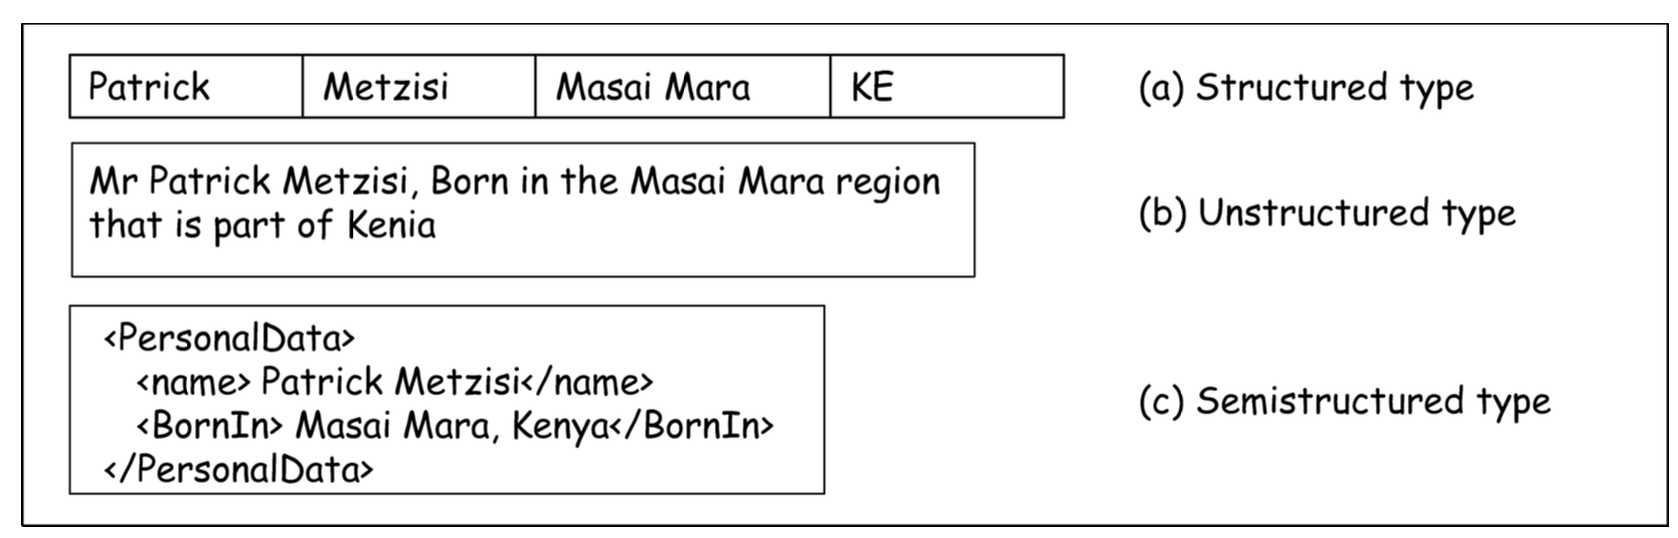
\includegraphics[width=1\textwidth]{Paper/figures/DataType.png}
    \caption{Data Type.}
    \label{fig:datatype}
  \end{figure}

 Data quality techniques become increasingly complex as data lose structure. For example, let us consider a registry describing personal information such as Name, Surname, Region, and StateOfBirth. Figure \ref{fig:datatype} shows the representation of Mr. Patrick Metzisi, born in the Masai Mara region in Kenya, by using a structured Figure \ref{fig:datatype}(a), unstructured (Figure \ref{fig:datatype}(b)), and semistructured (Figure \ref{fig:datatype}(c)) type of data.
 The same quality dimension will have different metrics according to the type of data. This would be explained in later subsection.
 The large majority of research contributions in the data quality literature focuses on structured and semistructured data. For this reason, this report focuses on structured and semistructured data.

\subsection{Data Quality Problems}\label{sec:DataQualityProblems}
The data quality problem could be classified into four categories depending on two factor: context-independence and role perspective \cite{Borek2011AClassficationOfDataQualityAssessmentMethod}.
 Table \ref{table:DataQualityProblem} provides a brief definition for each DQ problem.
 In the context independent category, spelling errors, missing data, and incorrect values are self-explanatory DQ problems.
 Duplicate data problems occur when rows are duplicated or when schemas contain redundancies.
 Data format problems occur when two or more semantically equivalent data values have different representations, including inconsistent and text formatting.
 Syntax violation problems occur when a pre-specified format has been assigned to an attribute and a data value for this attribute does not adhere to this format, including incomplete data format.
 Problems with violations of integrity constraints arise when data values do not adhere to pre-specified database integrity constraints; we also therefore include unique value violations, rather than have these as a separate problem, because unique value violations are one type of database integrity constraint.
 Note that, despite its position in Table we treat outdated data to be a user perspective problem because whether data is out of date depends on the purpose it is used for.

 For the context dependent category, the problem of violation of domain constraints is when an attribute value must be in a pre-specified context-dependent domain of values.
 Violation of organizational business rules is when any set of values do not adhere to a pre-specified rules assigned by the organization.
 Violation of company and governmental regulations is when any set of values do not adhere to a prespecified rules assigned imposed on the organization by legislating bodies.
 Similarly, violation of constraints provided by the database administrator is when any set of values do not adhere to a pre-specified rules assigned by the database administrator. In \ref{sec:DataQualityDimensions}, the problems are define in different dimensions with specific indicators.

 % Please add the following required packages to your document preamble:
% \usepackage[normalem]{ulem}
% \useunder{\uline}{\ul}{}
\begin{table}[]
\begin{tabular}{l|l|l|}
\cline{2-3}
                                                                                     & Data Perspective                                                                                                                                                                                                                                                             & User Perspective                                                                                                                                                                                                                                                                                                                                                                \\ \hline
\multicolumn{1}{|l|}{\begin{tabular}[c]{@{}l@{}}Context-\\ independent\end{tabular}} & \begin{tabular}[c]{@{}l@{}}Spelling error\\ Missing data\\ Duplicate data\\ Incorrect value\\ Inconsistent data format Outdated data\\ Incomplete data format\\ Syntax violation\\ Unique value violation Violation of \\ integrity constraints Text formatting\end{tabular} & \begin{tabular}[c]{@{}l@{}}The information is inaccessible\\ The information is insecure\\ The information is hardly retrievable \\ The information is difficult to aggregate\\ Errors in the information transformation\end{tabular}                                                                                                                                           \\ \hline
\multicolumn{1}{|l|}{\begin{tabular}[c]{@{}l@{}}Context-\\ dependent\end{tabular}}   & \begin{tabular}[c]{@{}l@{}}Violation of domain constraints \\ Violation of organization's business rules\\ Violation of company and government\\ regulations \\ Violation of constraints provided by\\  the database administrator\end{tabular}                              & \begin{tabular}[c]{@{}l@{}}The information is not based on fact \\ The information is of doubtful credibility\\ The information presents an impartial view\\ The information is irrelevant to the work\\ The information is incomplete\\ The information is compactly represented\\ The information is hard to manipulate \\ The information is hard to understand\end{tabular} \\ \hline
\end{tabular}
\caption{Types of Data Quality Problem}
\label{table:DataQualityProblem}
\end{table}


\subsection{Data Quality Dimensions}\label{sec:DataQualityDimensions}

To define data quality dimension, a data quality is proposed, as shown in Figure \ref{fig:twolayerstandard}. With each dimension, there is underlying data qulity elements and indicators.
In \citet{Cai2005ChallnegesOfDataQuality}, they chose data quality dimensions commonly accepted and widely used as big data quality standards and redefined their basic concepts based on actual business needs.
Each dimension was divided into many typical elements associated with it, and each element has its corresponding quality indicators: Accessibility
, Timeliness
, Authorization
, Credibility
, Definition/Documentation
, MetaData
, Accuracy
, Consistency
, Integrity
, Completeness
, Auditability
, Fitness
, Readability
, and Structure.
In this way, hierarchical quality standards for big data were used for evaluation.
Figure \ref{fig:twolayerstandard} shows a universal two-layer data quality standard. Detailed correspondence dimension, element and indicators are shown in Figure \ref{fig:hierachicalframwork}.

  \begin{figure}
    \centering
    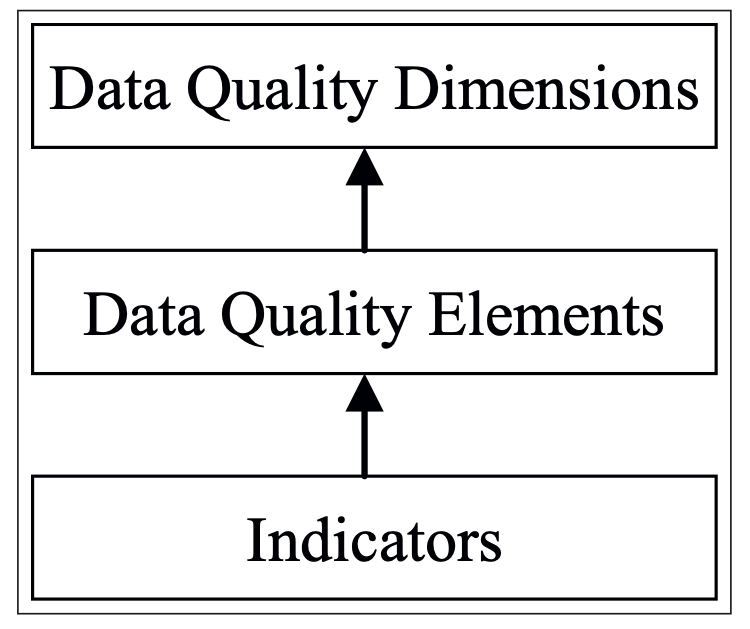
\includegraphics[width=0.25\textwidth]{Paper/figures/DataQualityFramework.png}
    \caption{Data quality framework.}
    \label{fig:dataqualityframework}
  \end{figure}

  \begin{figure}
    \centering
    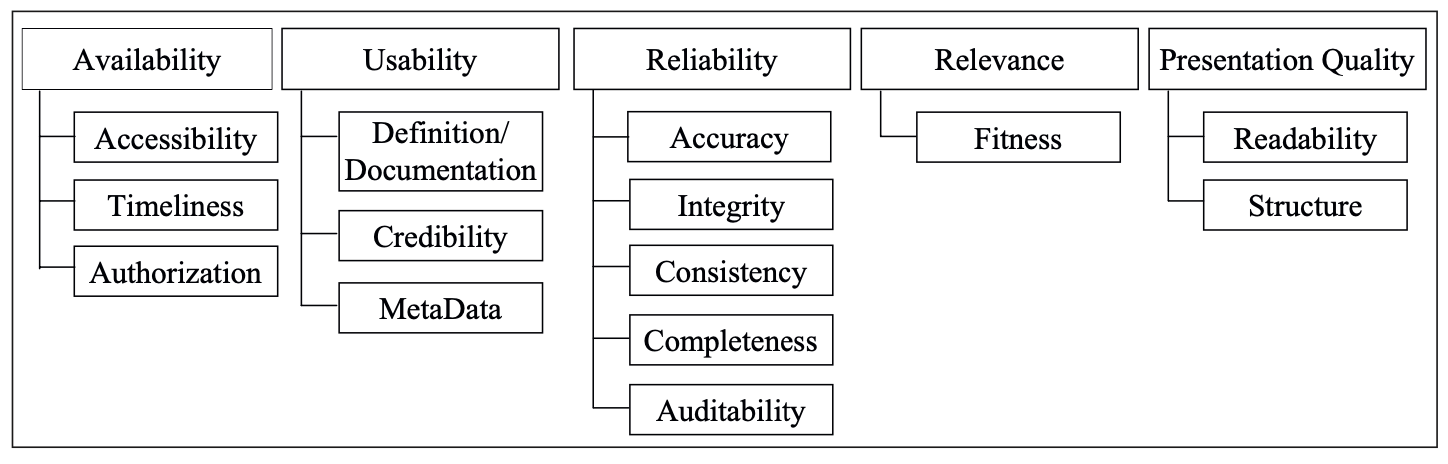
\includegraphics[width=1\textwidth]{Paper/figures/TwoLayerStandard.png}
    \caption{A universal, two-layer big data quality standard for assessment.}
    \label{fig:twolayerstandard}
  \end{figure}

\begin{figure}
    \centering
    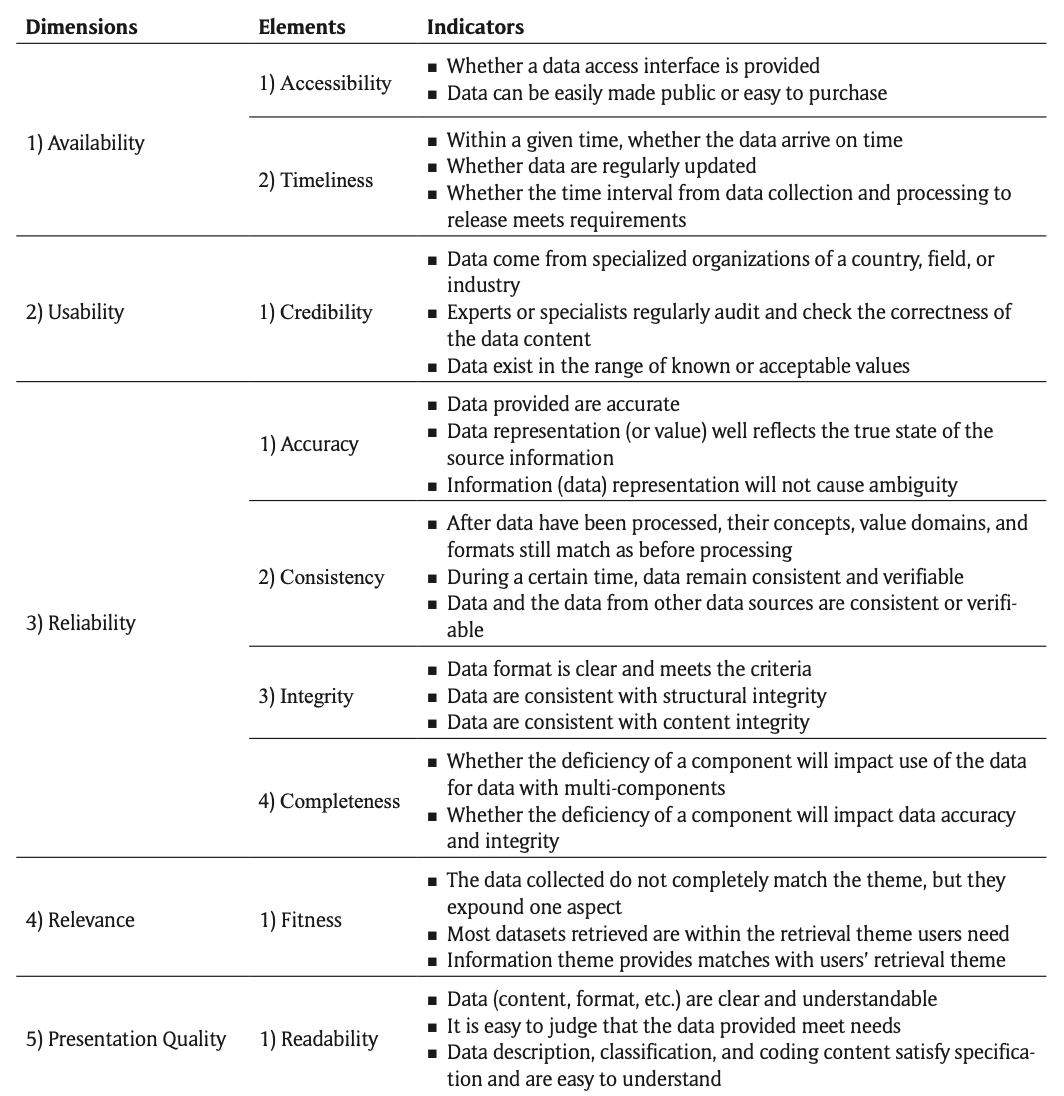
\includegraphics[width=1\textwidth]{Paper/figures/HierarchicalFrameWork.png}
    \caption{The hierarchical big data quality assessment framework(partial content).}
    \label{fig:hierachicalframwork}
 \end{figure}
Under the same dimension and elements, the indicators varies with type of data structure.
 For instance, syntactic accuracy is measured as described in Section \ref{sec:DataTypes} in the case of structured data. With semistructured data, the distance function should consider a global distance related to the shape of the XML tree in addition to the local distance of fields.

\section{Assessment Methodology Overview}

\subsection{Phases and Steps}
In the most general case, the sequence of activities of a data quality methodology is composed of three phases \cite{Batini2009MethodologiesForDataQuality}:

\begin{enumerate}
    \item \textbf{State Reconstruction}, which is aimed at collecting contextual information on organizational processes and services, data collections and related management procedures, quality issues and corresponding costs; this phase can be skipped if contextual information is available from previous analyses.
    \item \textbf{Assessment}, which measures the quality of data collections along relevant quality dimensions; the term measurement is used to address the issue of measuring the value of a set of data quality dimensions.
    \item \textbf{Improvement}, which concerns the selection of the steps, strategies, and techniques for reaching new data quality targets.
\end{enumerate}

\begin{comment}
The term assessment is used when such measurements are compared to reference values, in order to enable a diagnosis of quality. The term assessment is adopted in this article, consistent with the majority of methodologies, which stress the importance of the causes of poor data quality.
\end{comment}

\subsubsection{Assessment Steps}
includes:
(1) Data Analysis, which examines data schemas and performs interviews to reach a complete understanding of data and related architectural and management rules;
(2) DQ Requirements Analysis, which surveys the opinion of data users and administrators to identify quality issues and set new quality targets;
(3) Identification of Critical Areas, which selects the most relevant databases and data flows to be assessed quantitatively;
(4) Process Modeling, which provides a model of the processes producing or updating data;
(5) Measurement of Quality, which selects the quality dimensions affected by the quality issues identified in the DQ requirements analysis step and defines corresponding metrics.
\begin{comment}
measurement can be objective when it is based on quantitative metrics, or subjective, when it is based on qualitative evaluations by data administrators and users.
\end{comment}

\subsubsection{Improvement Steps}
includes:
(1) Evaluation of Costs, which estimates the direct and indirect costs of data quality;
(2) Assignment of Process responsibilities, which identifies the process owners and defines their responsibilities on data production and management activities;
(3) Assignment of Data Responsibilities, which identifies the data owners and defines their data management responsibilities;
(4) Identification of the Causes of Errors, which identifies the causes of quality problems;
(5) Selection of Strategies and Techniques, which identifies all the data improvement strategies and corresponding techniques, that comply with contextual knowledge, quality objectives, and budget constraints;
(6) Design of Data Improvement Solutions;
(7) Process Control;
(8) Process Redesign;
(9) Improvement Management;
(10) Improvement Monitoring;

\begin{comment}
(6) Design of Data Improvement Solutions, which selects the most effective and efficient strategy and related set of techniques and tools to improve data quality;
(7) Process Control, which defines check points in the data production processes, to monitor quality during process execution;
(8) Process Redesign, which defines the process improvement actions that can deliver corresponding DQ improvements;
(9) Improvement Management, which defines new organizational rules for data quality;
(10) Improvement Monitoring, which establishes periodic monitoring activities that provide feedback on the results of the improvement process and enables its dynamic tuning.
\end{comment}
Note that in all the steps of the assessment phase, a relevant role is played by metadata that store complementary information on data for a variety of purposes, including data quality. Metadata often provide the information necessary to understand data and/or evaluate them.

\subsection{Strategies and Techniques}
There are two types of strategies: data-driven and process-driven. Data-driven strategies improve the quality of data by directly modifying the value of data and Process-driven strategies improve quality by redesigning the processes that create or modify data.

\subsubsection{Data-Driven Techniques}
includes
\begin{enumerate}
    \item Acquisition of New Data, which improves data by acquiring higher-quality data to replace the values that raise quality problems.
    \item Standardization, which replaces or complements nonstandard data values with corresponding values that comply with the standard. For example, nicknames are replaced with corresponding names, for example, Bob with Robert, and abbreviations are replaced with corresponding full names, for example, Channel Str. with Channel Street.
    \item Record Linkage, which identifies that data representations in two (or multiple) tables that might refer to the same real-world object;
    \item Data and Schema Integration, which define a unified view of the data provided by heterogeneous data sources. Integration has the main purpose of allowing a user to access the data stored by heterogeneous data sources through a unified view of these data.
    \item Source Trustworthiness, which selects data sources on the basis of the quality of their data;
    \item Error Localization and Correction, which identify and eliminate data quality errors by detecting the records that do not satisfy a given set of quality rules. These techniques are mainly in the statistical domain.
    \item Cost optimization, defines quality improvement actions along a set of dimensions by minimizing costs.
\end{enumerate}

\begin{comment}
 Heterogeneities can be classified into technological heterogeneities, schema heterogeneities,and instance-level heterogeneities.
In distributed, cooperative, and P2P information systems data sources are characterized by various kinds of heterogeneities that can be generally classified into

(1) technological heterogeneities, (2) schema heterogeneities, and (3) instance-level heterogeneities.
Technological heterogeneities are due to the use of products by different vendors, employed at various layers of an information and communication infrastructure.
Schema heterogeneities are primarily caused by the use of (1) different data models, as in the case of a source that adopts the relational data model and a different source that adopts the XML data model, and (2) different representations for the same object, such as two relational sources that represent an object as a table and an attribute. Instance-level heterogeneities are caused by different, conflicting data values provided by distinct sources for the same objects. For instance, this type of heterogeneity can be caused by independent and poorly coordinated processes that feed the different data sources.
Data integration must face all the types of these listed heterogeneities.
\end{comment}

\subsubsection{Process-Driven Techniques}
- Process control inserts checks and control procedures in the data production process when: (1) new data are created, (2) data sets are updated, or (3) new data sets are accessed by the process. In this way, a reactive strategy is applied to data modification events, thus avoiding data degradation and error propagation.
- Process redesign redesigns processes in order to remove the causes of poor quality and introduces new activities that produce data of higher quality.
\begin{comment}
\subsubsection{Techniques}
 - Column analysis: Number of (unique) values and the number of instances per value as percentage from the total number of instances in that column
 - Cross-domain analysis
 - Data validation
 - Domain analysis
 - Lexical analysis
 - Matching algorithms: identify duplicates
 - Primary key and foreign key analysis (PK/FK analysis) : are good candidates for a PK/FK
 - Schema matching: two attributes are semantically equivalent
 - Semantic profiling
\end{comment}

\subsection{Cost}
The cost of a data quality program can be considered a preventive cost that is incurred by organizations to reduce data errors. This cost category includes the cost of all phases and steps that compose a data quality assessment and improvement process.
 The costs of poor quality can be classified as:
\begin{itemize}
    \item Process Costs, such as the costs associated with the re-execution of the whole process due to data errors;
    \item Opportunity Costs, which is due to lost and missed revenues.
\end{itemize}
 The cost of poor data quality is strongly context-dependent as opposed to the cost of a data quality program. This makes its evaluation particularly difficult, as the same data value and corresponding level of quality has a different impact depending on the recipient. For example, an active trader receiving obsolete information on a stock may incur considerable economic losses as a consequence of wrong investment decisions. In contrast, a newspaper receiving the same obsolete information to publish monthly trading reports may not experience any economic loss.

\subsection{Classification of Methodologies}
We can classify these methodologies into 3 categories based on their emphasis on improvement, assessment, cost and quality dimensions.  The categories are:
\begin{enumerate}
    \item Complete methodologies, which provide support to both the assessment and improvement phases, and address both technical and economic issues;
    \item Audit methodologies, which focus on the assessment phase and provide limited support to the improvement phase;
    \item Operational methodologies, which focus on the technical issues of both the assessment and improvement phases, but do not address economic issues.
    \item Economic methodologies, which focus on the evaluation of costs.
\end{enumerate}

Figures \ref{fig:classificationMethodologies} show the methods positioned on a two-dimensional coordinated.

\section{Case Study: Total Data Quality Management (TDQM)}\label{sec:TDQM}
 \cite{Bowo2019CaseStudy}

This section introduces the TDQM methodology and its applications.  The reason TDQM is chosen as a case study is that TDQM is a complete and general-purpose methodology. It also suggests a complete set of relevant dimensions and improvement methods that can be applied in different contexts.
The TDQM methodology was the first general methodology published in the data quality literature. \cite{Wang1998TDQM}
TDQM’s goal is to support the entire end-to-end quality improvement process, from requirements analysis to implementation.
TDQM is based on the principles of Total Quality Management (TQM). \cite{OAKLAND1999TQM}  In the original paper, the word Information is used instead of Data. For convenience, these two words will be used interchangeably. TDQM proposes a language for the description of information production (IP) processes.  It identifies four roles for the IP process:
\begin{itemize}
    \item information suppliers, which create or collect data for the IP,
    \item information manufacturers, which design, develop, or maintain data and related system infrastructure,
    \item information consumers, which use data in their work,
    \item information process managers, which are responsible for managing the entire information production process throughout the information life cycle.
The roles are responsible for the different phases of the quality improvement process.
\end{itemize}
\subsection{Data Types and Quality Dimensions}
TDQM supports both structured and semistructured data typed. It refers to DQ as Information Quality (IQ) and categorized them into four categories as shown in Table \ref{table:TDQMIQcatergories}.

\begin{table}[]
\centering
\begin{tabular}{|c|c|}
\hline
IQ Category         & IQ Dimensions                                                                                                                        \\ \hline
Intrinsic IQ        & Accuracy, Objectivity, Believability, Reputation                                                                                     \\ \hline
Accessibility IQ    & Access, Security                                                                                                                     \\ \hline
Contextual IQ       & \begin{tabular}[c]{@{}c@{}}Relevancy, Value-Added, Timeliness,\\ Completeness, Amount of data\end{tabular}                           \\ \hline
Representational IQ & \begin{tabular}[c]{@{}c@{}}Interpretability, Ease of understanding, Concise\\ representation, Consistent representation\end{tabular} \\ \hline
\end{tabular}
\caption{Information quality categories and dimensions}
\label{table:TDQMIQcatergories}
\end{table}

\subsection{Phases and Steps}

The TDQM has four cycles: defining, measuring, analyzing,
and improving IQ. A schematic of the TDQM methodology is shown in Figure. The tasks embedded in the methodology are performed iteratively to ensure high-quality IP. The Definition, Measurement, and  Analysis cycle are considered as the assessment phase introduced in the section.  The last cycle is the improvement phase.
\begin{enumerate}
    \item Definition: Data analysis,  DQ requirements analysis, process modeling are performed in this phase. The input of this phase is IP. The output consists of three-part:
    \begin{itemize}
        \item The logical and physical design of the Information Product with the necessary quality attributes
        \item A quality entity-relationship model that defines the IP and its IQ requirements
        \item An information manufacturing system that describes how the IP has been produced
    \end{itemize}
    Define IP Characteristics is a  data analysis task. It defines characteristics at two levels: (1) high level: description of functionalities for information consumers
(2) low-level description of the basic units and components of the information product and their relationships
Define IQ Requirements is a DQ requirements analysis. It defines the IQ requirements from the perspective of four roles of IP:  suppliers, manufacturers, consumers, and managers.
Define Information Manufacturing System is a process modeling task.
TDQM uses an information production map, IP-MAP, a graphical model designed to help them to visualize the information production process.
    \item  Measurement: The input of this phase is IQ dimensions from the definition phase. The output is IQ problems. The main tasks are Definition of the IQ metrics and measurement of IP
    \item Analysis: The Inputs are IQ problems. Outputs are actions for improving data quality. The main task is to Analyze IP. The purpose is to identify the causes of errors and discrepancies.
    \item Improvement: Inputs are  IQ metrics. Outputs are IQ improvement techniques. The main task is to Improve IP. It identifies key areas for improvement and selects suitable strategies, and techniques.
\end{enumerate}
\subsection{Strategies and Techniques}
TDQM focus on process-driven strategies and techniques. TDQM provides guidelines to apply process-driven strategies by using the Information Manufacturing Analysis Matrix\cite{Ballou1998ModelingInformation}, which suggests when and how to improve data. The description of processes is a mandatory activity, consistent with the general orientation of process-driven strategies. After modeling and assessing the information production process, new process control activities are identified, and/or process redesign decisions are taken.  Complex solutions such as IP-MAP cannot always be adopted due to their high costs and, in some cases, the practical unfeasibility of a thorough process modeling step. For this reason, other methodologies adopt less formal, but more feasible solutions.

\subsection{Example}

\subsection{Application}
TDQM has been applied to several areas. Early TDQM versions are reported in several U.S.A. Department of Defence (DoD) documents (see US Department of Defense [1994]). the methodology has been the basis for a law enforcement tool [Sessions 2007]. Other applications of TDQM performed at the DoD Medical Command for Military Treatment Facilities (MTF) are reported in Wang [1998] and Corey et al. [1996]. A claimed advantage of TDQM is that based on target payoffs, critical DQ issues, and the corresponding types of data, one can effectively evaluate how representative and comprehensive the DQ metrics are and whether this is the right set of metrics. This is the reason for its extensive application in different contexts, such as insurance companies, as described in \cite{Nadkarni2006} and  \cite{Patrick2005}.

Recent use of TDQM is found in [PAPER]. PT JAS is a non-bank financial institution engaged in sharia guarantee. The company's main business is managing risk. By using TDQM, companies can find out in advance the condition of the quality of company data and immediately formulate strategies and steps to improve and develop the quality of the data they have, so that data can be a useful and valuable asset. The company focus on aspects of confidentiality, integrity, and availability. With TDQM, the defined dimensions and measure result are as following:
\begin{itemize}
    \item Completeness: 66 fields found with a percentage of 99\% data completeness and 5 fields with a percentage of 27\% \~ 33\% meet the criteria
    \item Validity: 2 out of 9 fields of data did not meet the criteria with 0.59\% (v5) and 3.39\% (v6) error rate
    \item Accuracy: 4 out of 9 fields did not meet the criteria with  1.25\% (acc3), 3.08\% (acc5), 1.83\% (acc6), and 2.24\% (acc9)

\end{itemize}
TDQM provides a common framework for facilitating understanding in data improvement approach through data quality management .
Nowadays, there are also many contributions extending TDQM, by improving IP-MAP [Scannapieco et al. 2005; Shankaranarayanan and Wang 2007] or by proposing a TDQM based Capability Maturity Model [Baskarada et al. 2006].


\begin{figure}
    \centering
    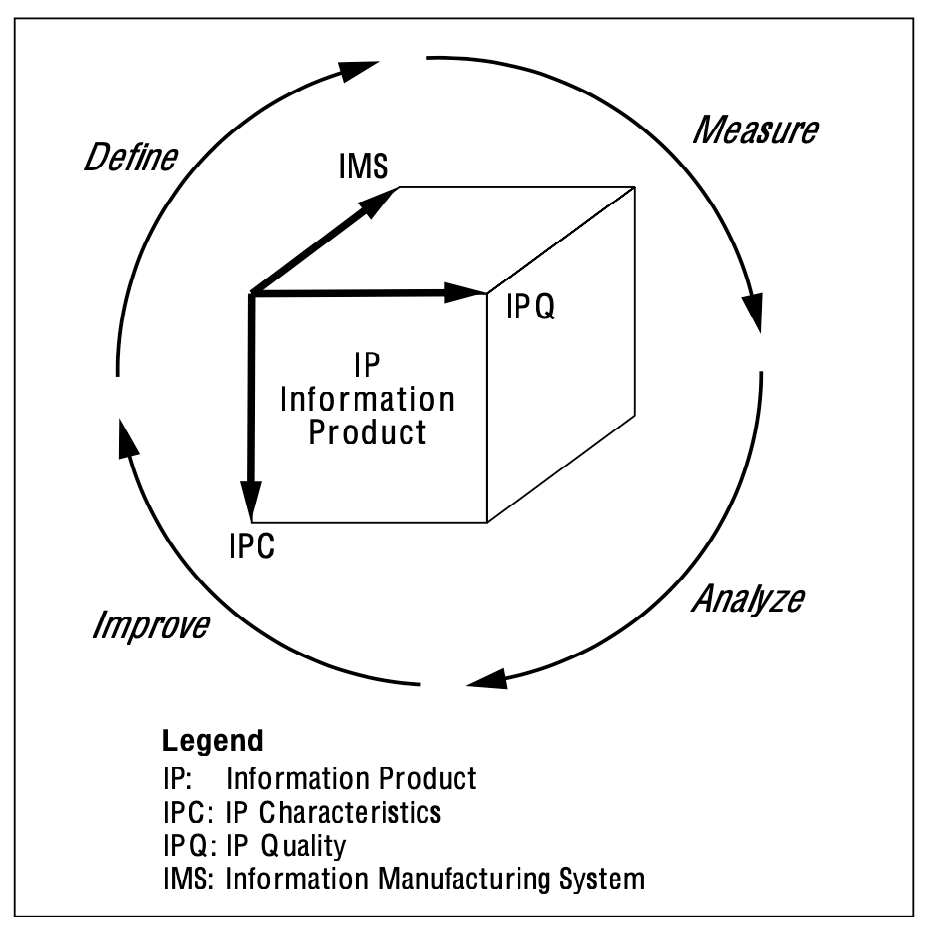
\includegraphics[width=0.5\textwidth]{Paper/figures/TDQM-2.png}
    \caption{TDQM Phases.}
    \label{fig:PhasesTDQM}
 \end{figure}


\section{Comprehensive Data Quality (CDQ)}

The CDQ methodology \cite{Batini2006DQConceptsMethodologiesTechniques} \cite{Batini2007ComprehensiveDQ} \cite{Batini2008ComprehensiveDQ} is conceived to be at the same time complete, flexible, and simple to apply.

\begin{comment}
Completeness is achieved by considering existing techniques and tools and integrating them in a framework that can work in both intra- and inter-organizational contexts, and can be applied to all types of data, structured, semistructured and unstructured.
The methodology is flexible since it supports the user in the selection of the most suitable techniques and tools within each phase and in any context.
Finally, CDQ is simple since it is organized in phases and each phase is characterized by a specific goal and set of techniques to apply.

In fact, the other methodologies implicitly assume that contextual knowledge has been previously gathered and modelled.
\end{comment}

The CDQ provides support to select the optimal quality improvement process that maximizes benefits within given budget limits and emphasizes the initial requirements elicitation phase.
The focus is on how to reach total data quality without providing indications as to how to use contextual knowledge. A goal of CDQ is instead to obtain a quantitative assessment of the extent to which business processes are affected by bad information.

\begin{figure}
    \centering
    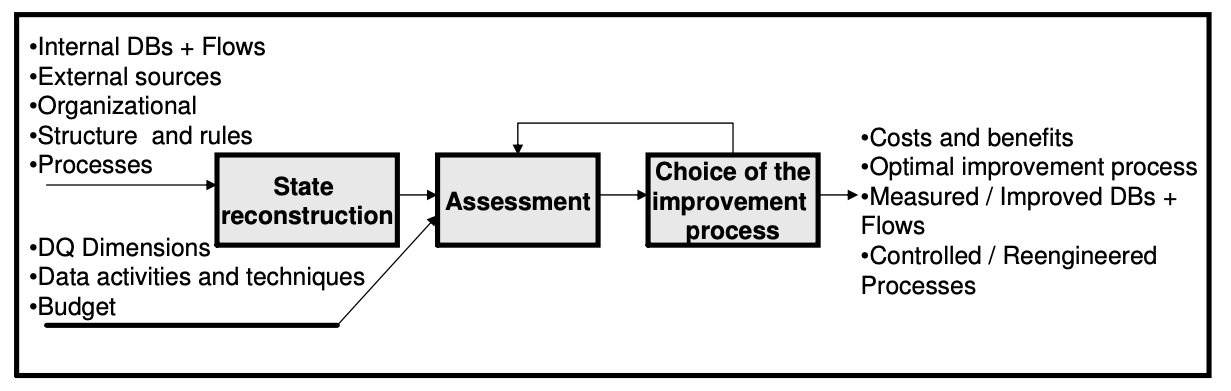
\includegraphics[width=1\textwidth]{Paper/figures/PhasesCDQ-2.png}
    \caption{CDQ Phases.}
    \label{fig:PhasesCDQ}
 \end{figure}

Three main phases characterize the methodology: state reconstruction, assessment, and choice of the optimal improvement process shown in Figure \ref{fig:PhasesCDQ}.
In the first phase of the methodology, the relationships among organizational units, processes, services, and data are reconstructed.
These relationships are modelled by using matrices that describe which organizational units use data and their roles in the different business processes.
Furthermore, in this phase, processes are described along with their contribution in the production of goods/services and the legal and organizational rules that discipline workflows.
The second phase sets new target quality levels that are needed to improve process qualities, and evaluates corresponding costs and benefits.
This phase locates the critical variables affected by poor quality. Since improvement activities are complex and costly, it is advisable to focus on the parts of the databases and data flows that raise major problems.
Finally, the third phase consists of five steps and is aimed at the identification of the optimal improvement process: the sequence of activities that has the highest cost/effectiveness ratio.
New target quality levels are set by considering costs and benefits. Different improvement activities can be performed to reach new quality targets.
The methodology recommends the identification of all the data-driven and process-driven improvement techniques for the different databases affected by poor quality.
A set of mutually consistent improvement techniques constitutes an improvement process.
Finally, the most suitable improvement process is selected by performing a cost-benefit analysis.



  \begin{figure}
    \centering
    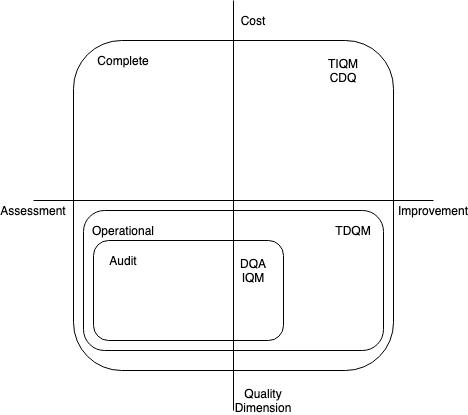
\includegraphics[width=0.75\textwidth]{Paper/figures/A classification of methodologies.png}
    \caption{A classification of methodologies.}
    \label{fig:classificationMethodologies}
  \end{figure}


\section{Conclusion}
This paper first introduces fundamentals of data quality, pipelines and classification of general assessment method, followed by the evaluation and analysis of five DQ assessment methods in term of different aspects.
Of all the surveyed methods, CDQ is considered to be the most complete, yet flexible, and simple to apply.
The completeness is achieved by considering existing techniques and tools and integrating them in a framework that can work in both intra- and inter-organizational contexts, and can be applied to all types of data, structured, semistructured and unstructured.
The methodology is flexible since it supports the user in the selection of the most suitable techniques and tools within each phase and in any context.
Experience suggests a “one size fits all” set of metrics is not a solution. The CDQ flexibility poses itself in great advantage over other methods.
Finally, CDQ is simple since it is organized in phases and each phase is characterized by a specific goal and set of techniques to apply.

The very motivation for this paper is to explore possibility of applying DQ assessment in academic research of software engineering, specifically CI/CD application. CI focuses on automation tools to allow development teams to integrate their efforts, build and test the code, while CD enables the code to be packaged and delivered with a fully automated deployment process. Both of the process are automated and generated logs and reports that are common in the format of semi-structured data, commonly stored in XML or HTML.
Therefore, the CDQ's capability of extension to other new metrics and flexibility make it the most suitable candidate for future application of DQ assessment in software engineering.

Two open issues are left to be investigated: DQ assessment method customized for specific information system and challenges in big data era.
From a historical perspective, there exists a correlation between quality dimensions and the evolution of ICT technologies.
The most critical issues with data quality management were error localization and correction in data sources, and record linkage between new data sources and preexisting data bases.
The evolution of information systems from monolithic to network-based has caused a growth of the number of data sources in both size and scope and, consequently has significantly increased the complexity of data quality management.

The characteristics of big data come down to the 4Vs: Volume, Velocity, Variety, and Value \cite{Katal2013BigData}. Volume refers to the tremendous volume of the data. Velocity means that data are being formed at an unprecedented speed and must be dealt with in a timely manner. Variety indicates that big data has all kinds of data types, and this diversity divides the data into structured data and unstructured data. These multityped data requires higher data processing capabilities.
Finally, Value represents low-value density. Value density is inversely proportional to total data size, the greater the big data scale, the less relatively valuable the data. Consequently, the cost of DQ assessment will gain significant importance is inevitable. How to accurately define and estimate the cost of DQ is another topic.

In the end, assessing data quality is an on-going effort that requires awareness of the fundamental principles underlying the development and context of application.

\bibliography{template}

\end{document}
